\documentclass{tstextbook}
\usepackage{color}
\usepackage{tabularx}
\usepackage{float}
\usepackage[dutch]{babel}
\definecolor{javared}{rgb}{0.6,0,0} % for strings
\definecolor{javagreen}{rgb}{0.25,0.5,0.35} % comments
\definecolor{javapurple}{rgb}{0.5,0,0.35} % keywords
\definecolor{javadocblue}{rgb}{0.25,0.35,0.75} % javadoc
\usepackage{pgffor, ifthen}
\usepackage{enumitem,amssymb}
\newlist{todolist}{itemize}{2}
\setlist[todolist]{label=$\square$}
\newcommand{\notes}[3][\empty]{%
    \noindent Notes\vspace{10pt}\\
    \foreach \n in {1,...,#2}{%
        \ifthenelse{\equal{#1}{\empty}}
            {\rule{#3}{0.5pt}\\}
            {\rule{#3}{0.5pt}\vspace{#1}\\}
        }
}
 
\lstset{language=Java,
basicstyle=\ttfamily,
frame=single,
breaklines=true,
keywordstyle=\color{javapurple}\bfseries,
stringstyle=\color{javared},
commentstyle=\color{javagreen},
morecomment=[s][\color{javadocblue}]{/**}{*/},
numbers=left,
numberstyle=\tiny\color{black},
stepnumber=2,
numbersep=10pt,
tabsize=4,
showspaces=false,
showstringspaces=false}

\newtheorem{envoefening}{Oefening}[chapter]
\newenvironment{oefening}
               {\begin{boxexercise}\begin{envoefening}}
               {\end{envoefening}\end{boxexercise}}
               
\newenvironment{todo}
{\vspace{0.5cm}\noindent
 \marginpar{\vspace{-3mm}
\includegraphics[width=1.0cm]{create.png}}}
{\vspace{0.5cm}}

\begin{document}

\tsbook{Java Advanced 2020-2021}
       {Nele Custers}
       {nvt}
       {2020}
       {xxxxx}{xxx--xx--xxxx--xx--x}{0.0}
       {Hogeschool PXL}
       {Hasselt}
       
\pagebreak

% Copyright page
\null
\vfill
\begin{flushleft}
  Copyright \copyright 2020 Nele Custers
  \vspace{5mm}
\end{flushleft}

%---------------------------------------------------------------------------
% Chapters
%---------------------------------------------------------------------------

%---------------------------------------------------------------------------


\renewcommand{\thesection}{\arabic{section}}

\chapter*{Streaming service}

\section{Aan de slag}

De github repository \url{https://github.com/custersnele/JavaAdvStreamingServiceV1} bevat een grafische userinterface (GUI) voor de streaming service.  De GUI is geschreven in JavaFX.

Fork dit project zodat je een eigen repository hebt waarmee je aan de slag kan gaan.
Je kan dit project daarna openen in IntelliJ IDEA. Dit project is een Maven project. 
Omdat we een JavaFX en nog enkele andere libraries nodig hebben,  is het interessant om Maven te gebruiken. Maven vergemakkelijkt het beheren van 3rd party libraries. Maven biedt nog veel meer dan enkel 3rd party libraries beheren in een project, maar dat valt buiten de scope van deze cursus. De 3rd party libraries die we gaan gebruiken vind je terug tussen de $<$dependencies$>$ tags in het bestand pom.xml. Dit bestand, het project object model (POM), bevat alle nodige configuratie voor Maven. 

Merk ook op dat Maven zijn eigen default mappenstructuur heeft.

\begin{figure}
  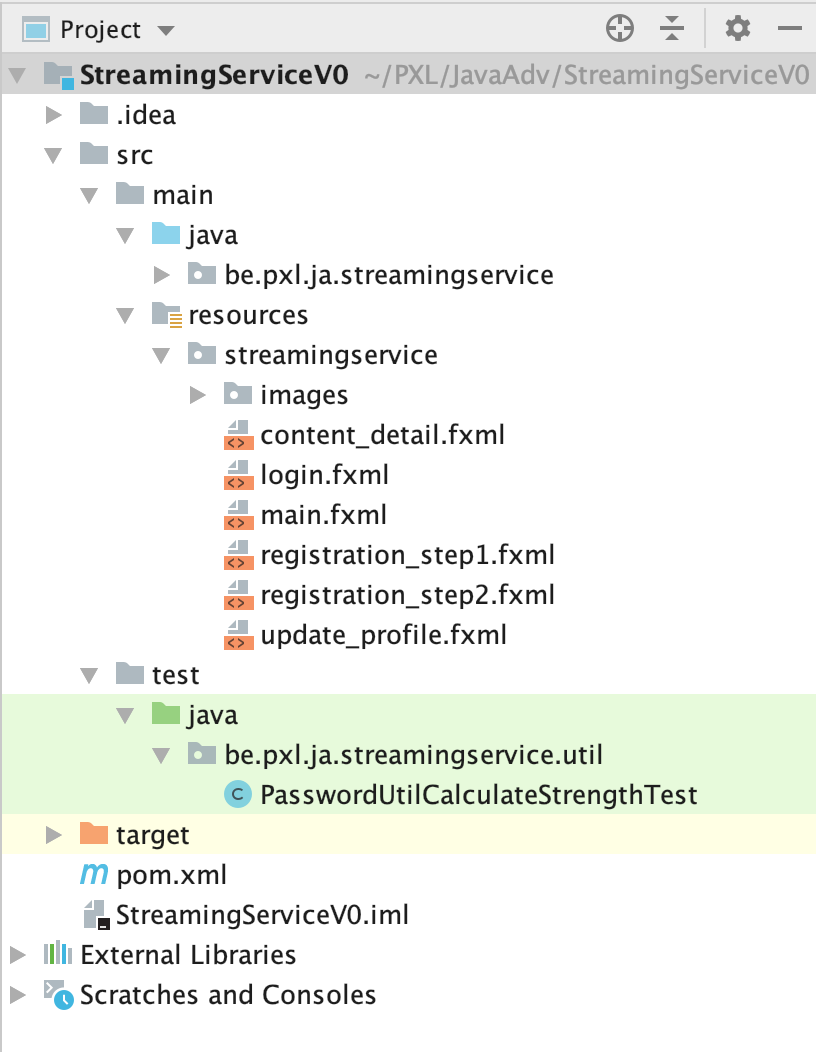
\includegraphics{images/h1/maven_project_structuur.png}
  \caption{Mappenstructuur van het maven project}
  \label{fig:maven_project_structure}
\end{figure}


Je ziet dat er nog veel compiler errors zijn in ons project. De code om de GUI te tonen en aan te sturen is reeds beschikbaar, maar we missen de klassen die we afgelopen weken reeds gedeeltelijk hebben ontwikkeld. 
\begin{theorem}
De klassen die je tot nu toe hebt ontwikkeld voor de streaming service voeg je toe in het package be.pxl.ja.streamingservice.model. Kopieer ook de bijhorende unit testen naar de juiste testfolder.  
\end{theorem}

We zullen nu alle klassen 1 voor 1 overlopen. Een aantal van de klassen heb je misschien al volledige ge\"implementeerd. Andere klassen moet je nog uitbreiden. De volledige beschrijving van alle klassen is gegeven, zodat je weet hoe je elke klasse moet implementeren. 
Een volledig klassendiagram vind je aan het einde van dit document.

\begin{figure}
  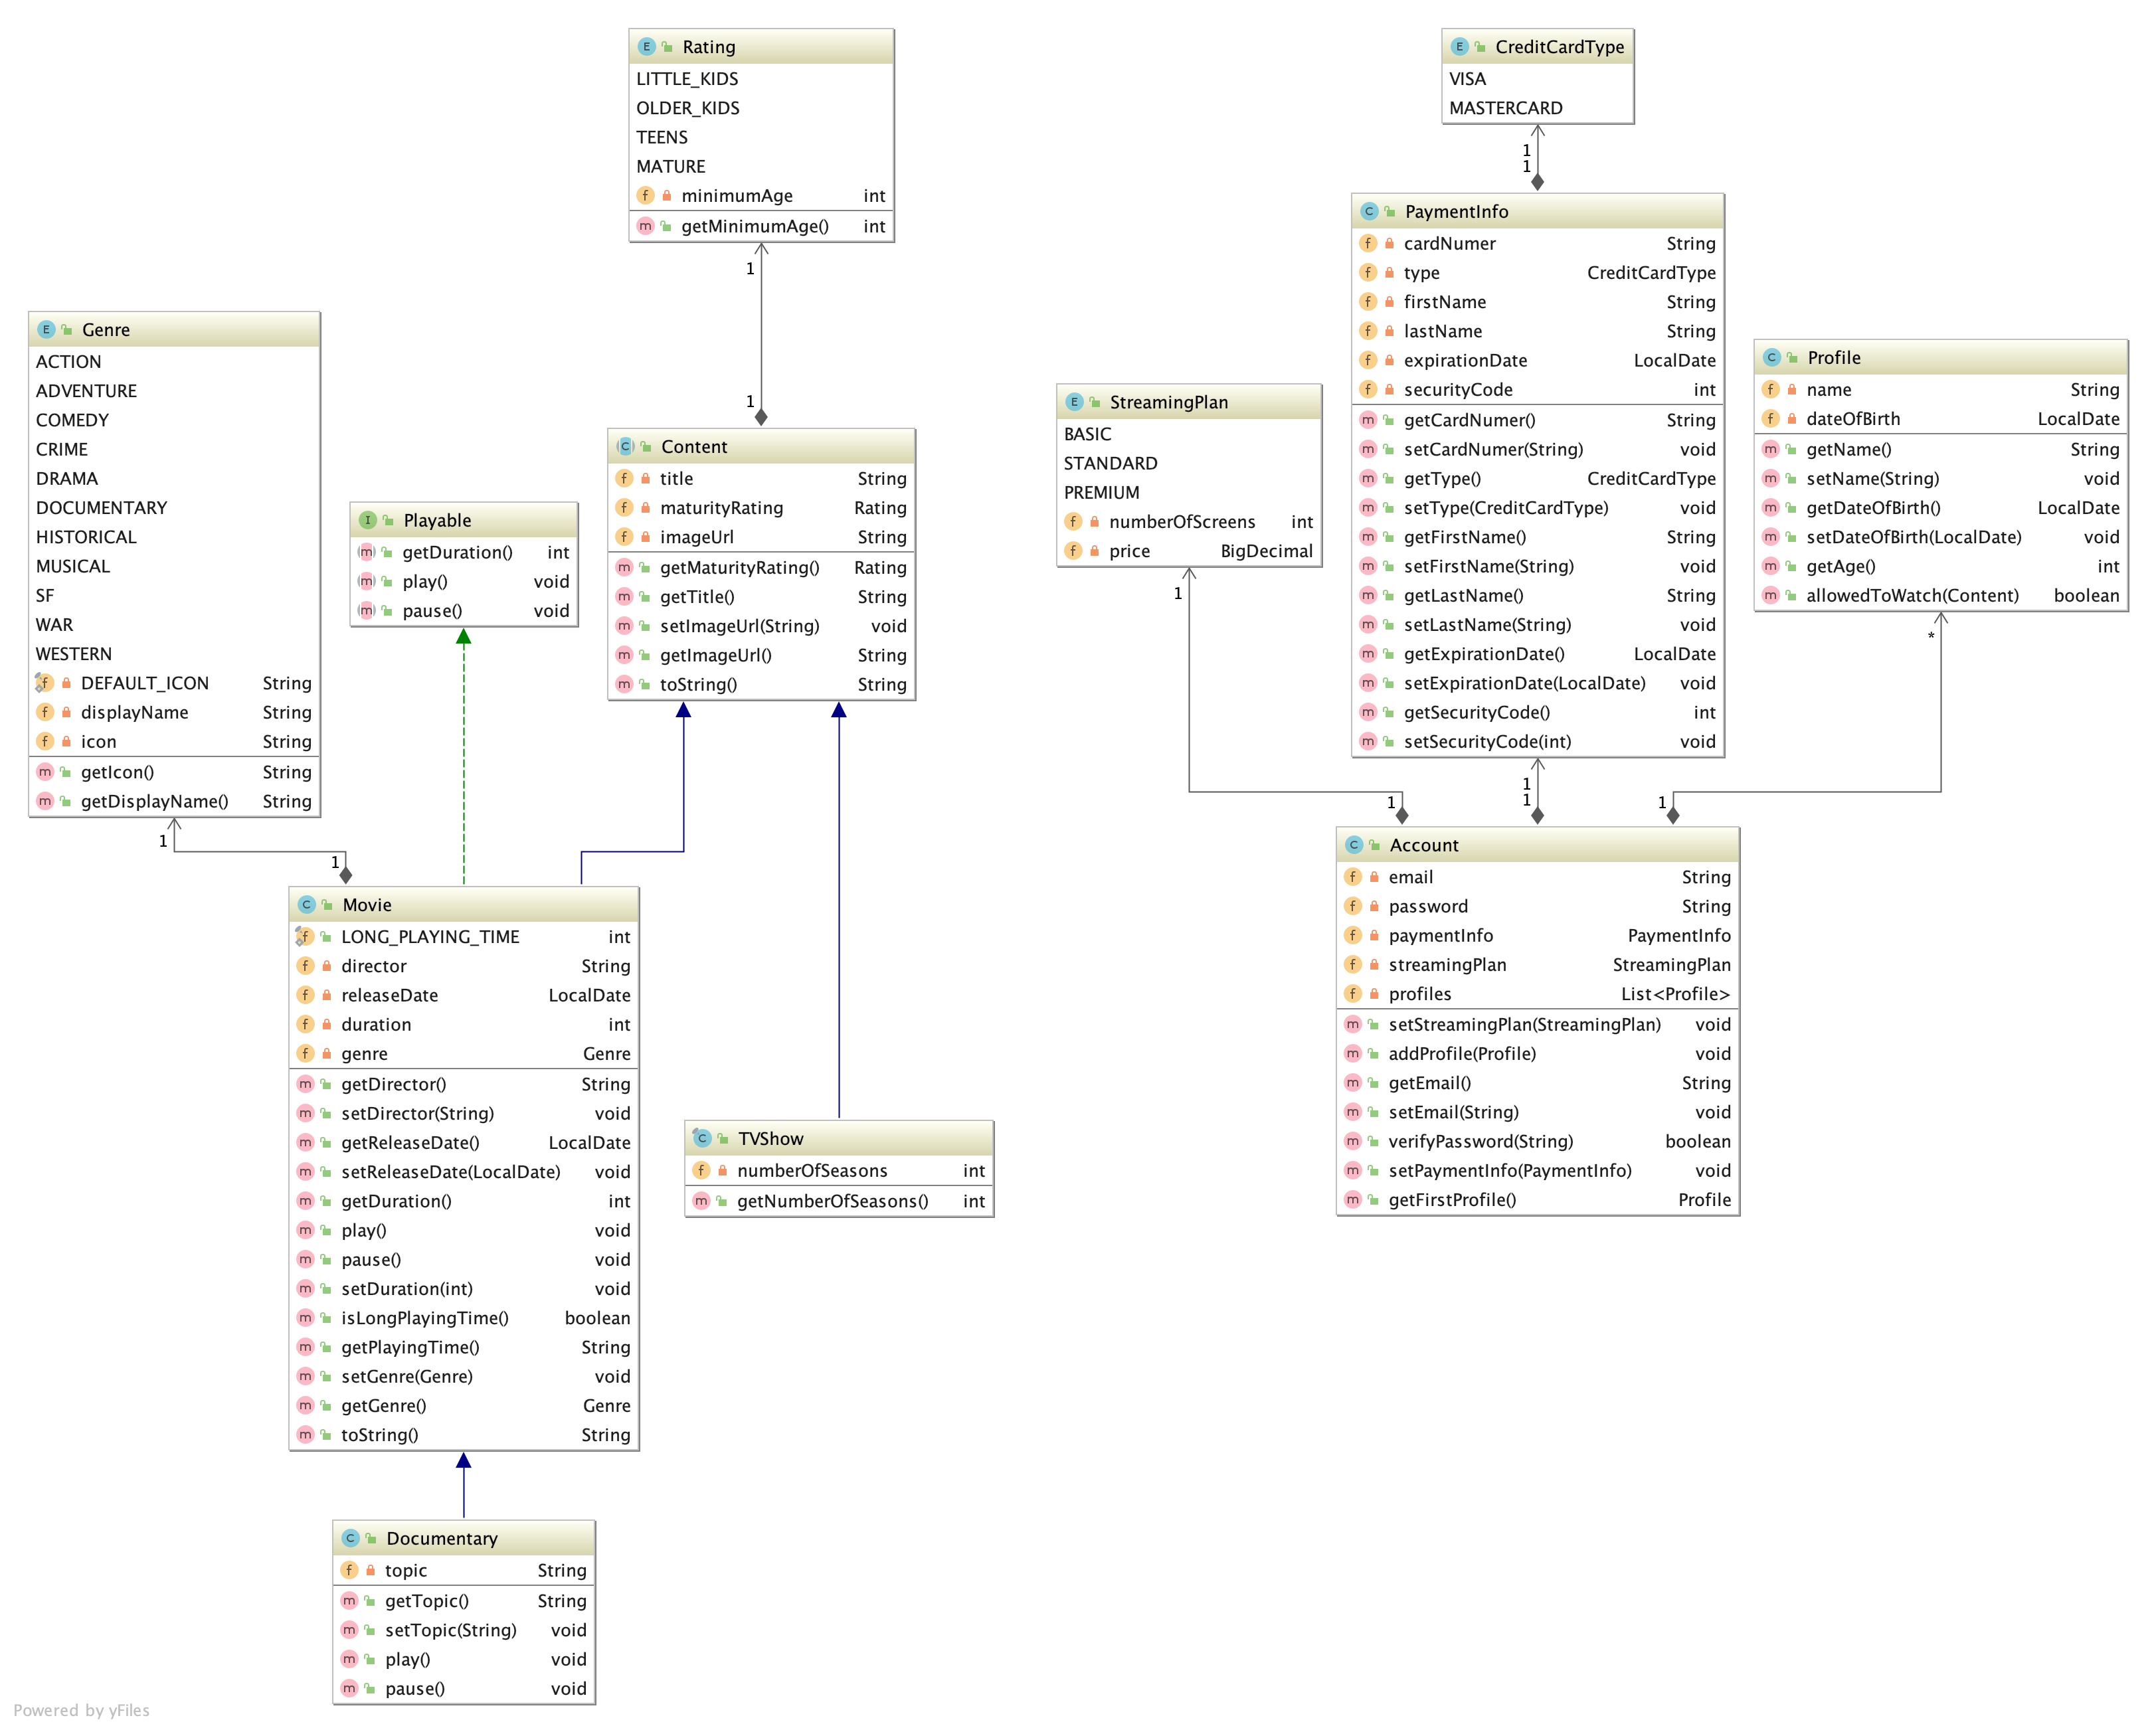
\includegraphics[width=\linewidth]{images/h1/streaming_service_v0.png}
  \caption{Klassen van de streaming service}
  \label{fig:streaming_service_class_diagram}
\end{figure}


\section{Profile}
We voegen in de klasse Profile een extra eigenschap toe: de eigenschap avatar (String). Pas ook de constructor van de klasse Profile aan. De constructor heeft nu 2 parameters: name en avatar. Voor een nieuw Profile-object is de geboortedatum null (niet ingevuld).

In de klasse Profile voorzie je drie verzamelingen voor Content-objecten: recent bekeken content (recentlyWatched), het materiaal wat momenteel wordt bekeken (currentlyWatching) en een verzameling met te bekijken content (My List of wachtlijst). Kies een gepaste klasse uit het Java Collection framework voor elke van deze verzamelingen. De methode startWatching in de klasse Profile zorgt ervoor dat de content \textbf{vooraan} in de verzameling currentlyWachting wordt toegevoegd. (Zorg er ook voor dat elk Content-object maar maximum 1 keer in de verzameling kan voorkomen.) De methode finishWatching() zorgt ervoor dat het Content-object niet meer voorkomt in de verzameling currentlyWachting, maar wel vooraan in de verzameling recentlyWatched wordt toegevoegd.

Er kan ook steeds content bij de wachtlijst toegevoegd of verwijderd worden. De methoden addToMyList() en removeFromMyList() moeten hiervoor gebruikt worden. Zorg dat er nooit Content-objecten meerdere keren in deze wachtlijst kunnen voorkomen.

Voorzie getters voor de 3 verzamelingen (recentlyWatched, currentlyWatching en myList).

\section{CreditCardType}

We hebben 2 soorten kredietkaarten die we aanvaarden: VISA en MASTERCARD. Kaartnummer op een visa-kaart start steeds met een ``4'',  kaartnummer van een Mastercard-kaart start altijd met een ``5''.  Het startnummer van de kaartnummer hou je ook bij in de enum-waarden.

\section{CreditCardNumber}

De klasse CreditCardNumber hebben we grotendeels ge\"implementeerd in het hoofdstuk Exceptions. Objecten van de klasse CreditCardNumber mogen nooit ongeldige gegevens bevatten. Wanneer je een object van de klasse CreditCardNumber probeert aan te maken met ongeldige gegevens zal er een IllegalArgumentException gegooid worden.
Zo wordt er steeds gecontroleerd dat een kaartnummer bestaat uit 16 cijfers en het controlegetal (cvc) uit 3 cijfers. Aan de hand van het kaartnummer kan ook het type van de kredietkaart afgeleid worden.

\section{PaymentInfo}

In de klasse PaymentInfo houden we alle gegevens die nodig zijn om maandelijks het abonnementsgeld voor de streaming service te betalen. De voornaam en achternaam op de kredietkaart alsook het kaartnummer (CreditCardNumber) en de vervaldatum van de kredietkaart worden bijgehouden. 
Bij de setter setExpirationDate controleer je dat de kredietkaart nog minstens \'e\'en maand geldig zal zijn. Indien dit niet het geval is, zal de InvalidDateException opgegooid worden. De InvalidDateException is een runtime exception. Meer info vind je ook bij oefening 3.7 in het hoofdstuk Exception handling.



\begin{figure}[H]
  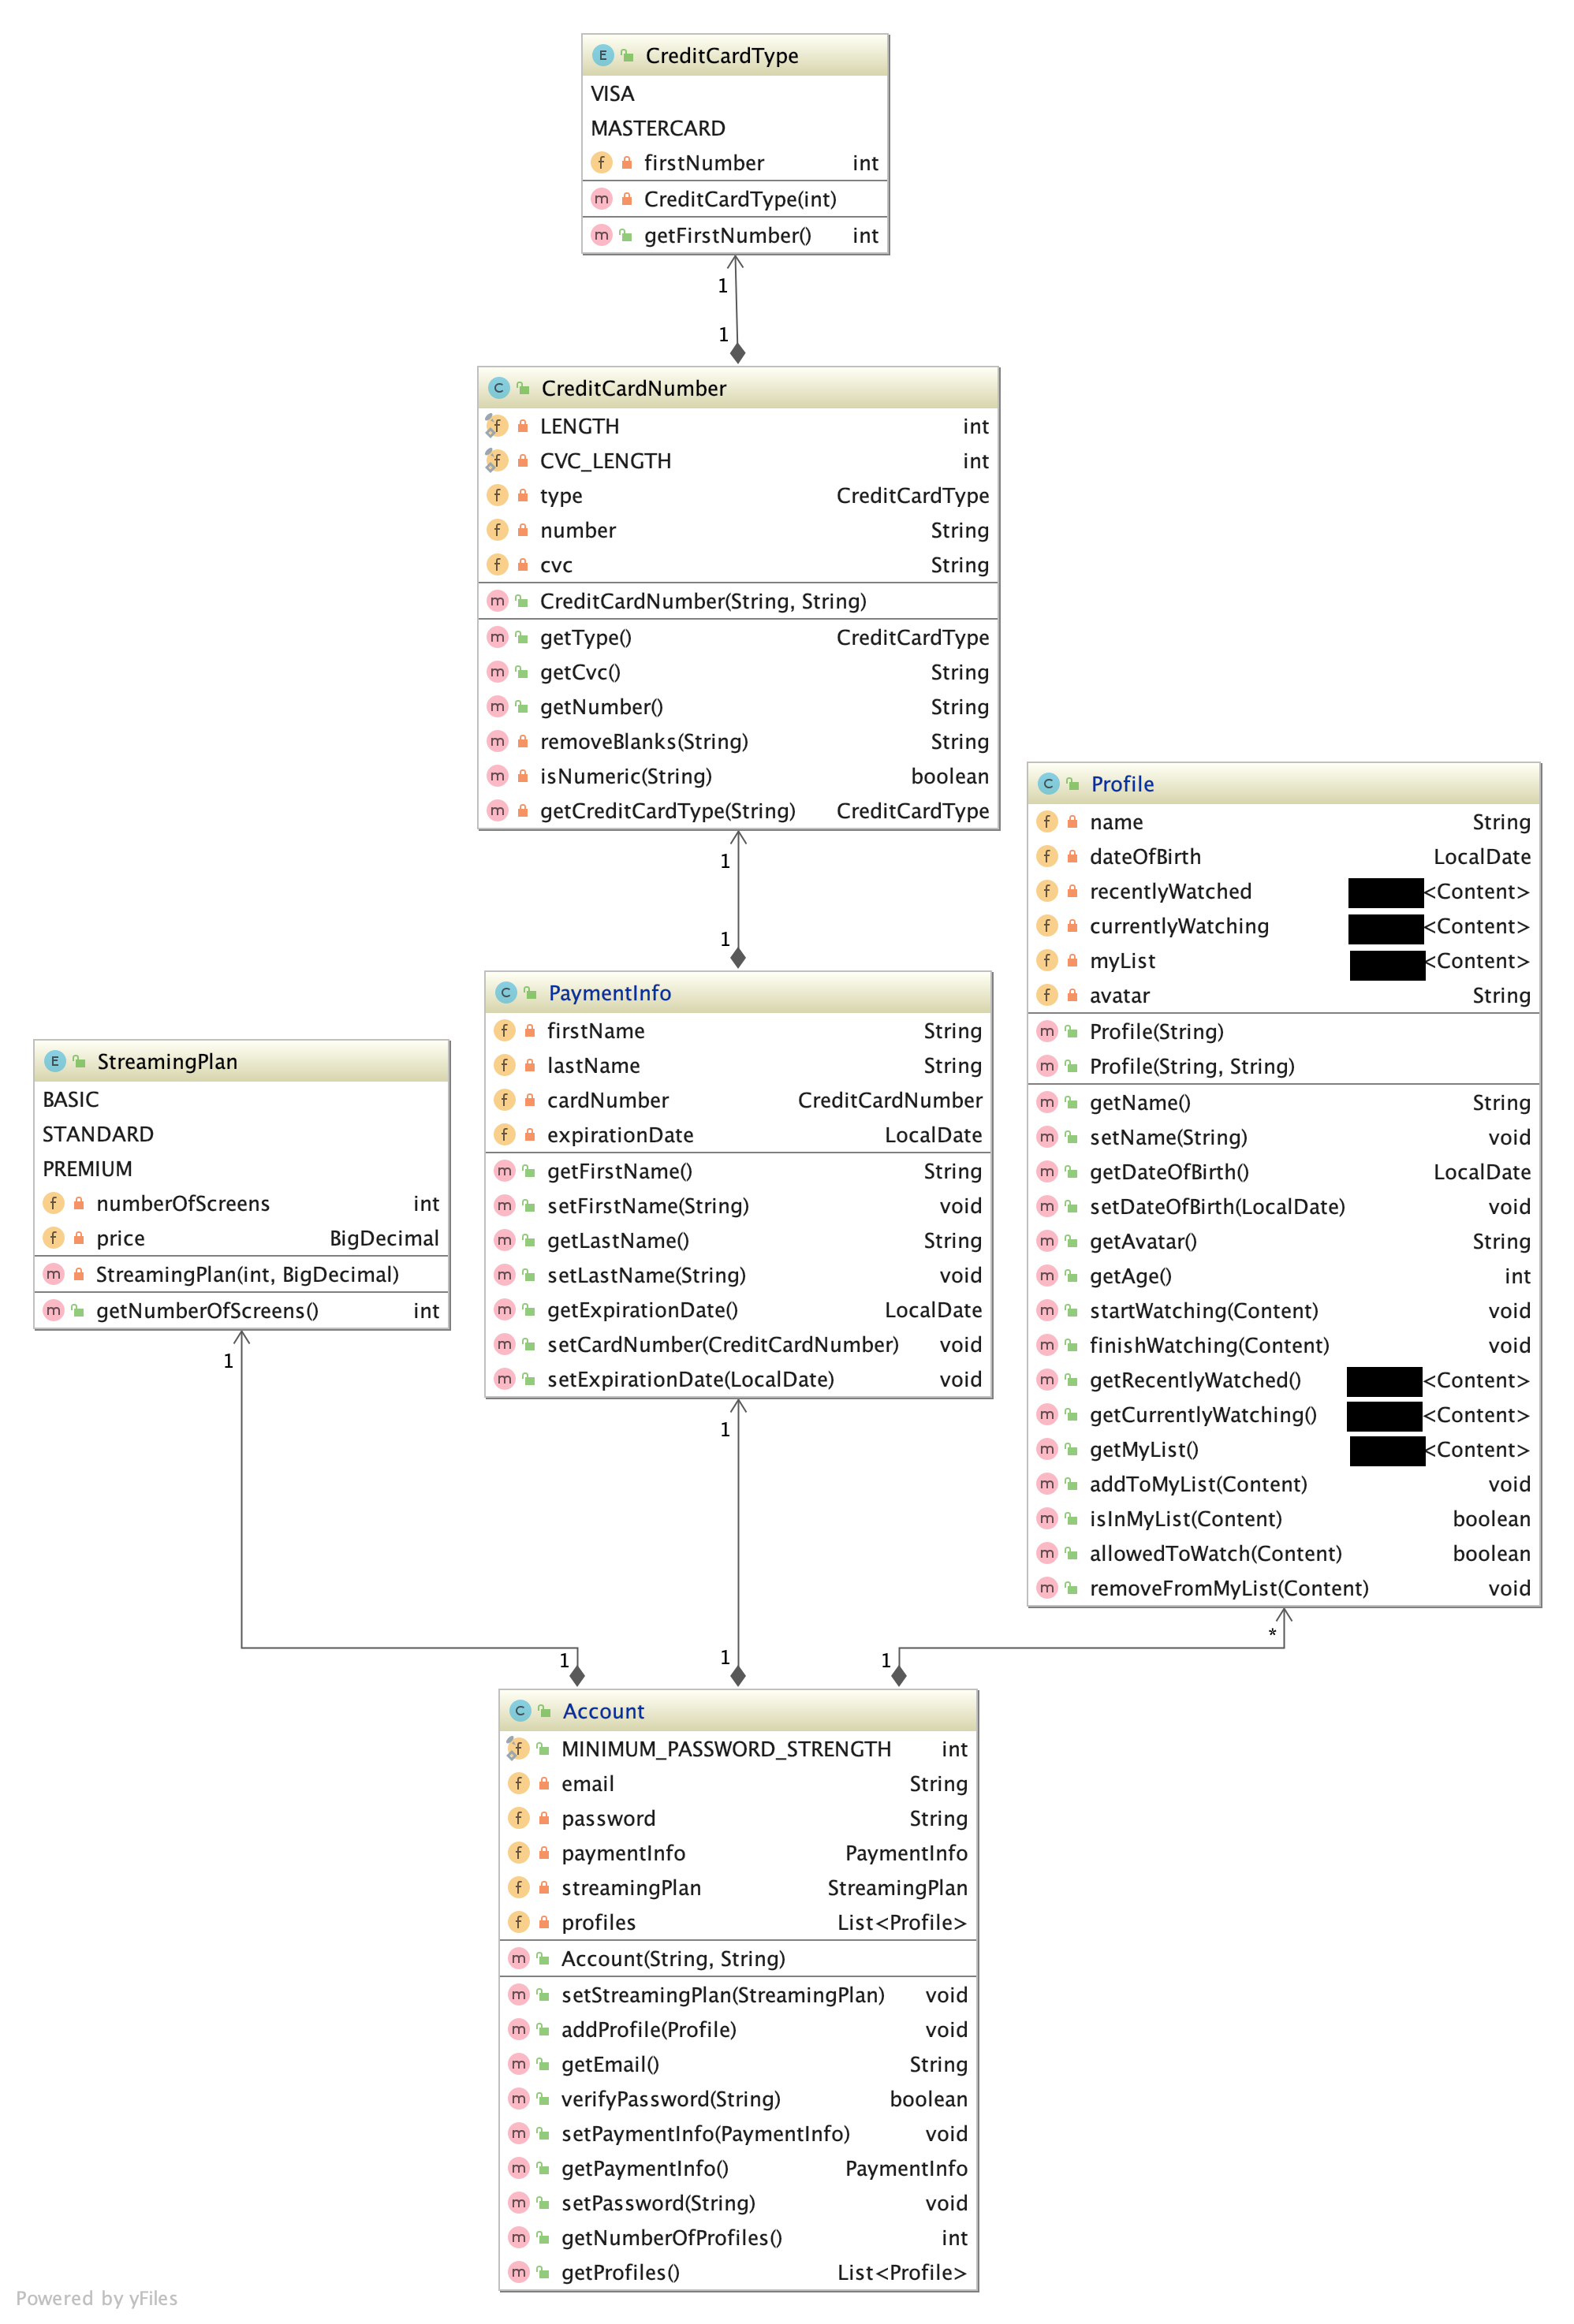
\includegraphics[height=\textheight]{images/diagrams/account_hierarchy.png}
  \caption{Klassen Account en associaties}
  \label{fig:content_hierarchy}
\end{figure}

\section{Account}
In de klasse Account kan een gebruiker, afhankelijk van het gekozen StreamingPlan, kijkprofielen toevoegen aan een Account. Gebruik een HashMap om deze Profile-objecten bij te houden. Hou rekening met het gekozen StreamingPlan als je een Profile-object toevoegt. Voorzie een unchecked exception TooManyProfilesException() die je opgooit als er geen extra Profile-objecten meer toegevoegd mogen worden. Gebruik de naam (name) van een Profile-object als key. Voorzie in de klasse Account een methode \textit{Profile getProfile(String name)}. Schrijf unit testen.




\section{Klasse Account en associaties}



\subsection{Profile}

Een profile heeft 3 eigenschappen: een naam (name), geboortedatum (dateOfBirth) en avatar. De avatar wordt gebruikt om een profiel-afbeelding te tonen. Bij de geboortedatum controleren we dat deze niet in de toekomst ligt (zie ook oefening 3.9).
Indien een geboortedatum in de toekomst wordt gegeven, gooi je een InvalidDateException.

De klasse Profile voorziet 2 constructoren. Een eerste constructor met 2 eigenschappen: name en avatar. Een tweede constructor voorziet 1 eigenschap: name, en geeft avatar de waarde ``profile1''.

I

\subsection{Account}

Ook in de klasse Account werden de afgelopen weken enkele aanpassingen uitgevoerd. Zo zal je in de constructor extra validaties moeten uitvoeren. De eigenschappen email en password zijn verplicht. Gooi een IllegalArgumentException indien de parameters voor deze eigenschappen \textit{null} of een lege string zijn. In de constructor wordt er ook een eerste kijkersprofiel aangemaakt met de naam ``Profile 1''.
StreamingPlan.BASIC wordt als default waarde voor een nieuw aangemaakt account toegekend. 

De methode setPassword gaat altijd controleren dat een gekozen wachtwoord een minimum sterkte van 5 heeft. De PasswordUtil, waarmee je de sterkte van een wachtwoord kan berekenen, is reeds aanwezig. Gooi opnieuw een IllegalArgumentException indien het paswoord niet de gewenste sterkte heeft.

Bij een account kunnen een aantal kijkersprofielen aangemaakt worden. Het aantal kijkerprofielen is afhankelijk van het gekozen StreamingPlan. Controleer in de methode addProfile() dat het aantal profielen het aantal toegelaten profielen van het gekozen StreamingPlan niet overschrijdt.
Je gooit een TooManyProfilesException wanneer het toegelaten aantal profielen wordt overschreden (zie ook oefening 4.6).

Zorg er ook voor dat de methode getProfiles() de Profile-objecten altijd gesorteerd op naam teruggeeft. 

Extra: zoek eens op hoe je kan controleren of een opgegeven e-mailadres wel degelijk een correct formaat heeft. Indien het e-mailadres een ongeldig formaat heeft gooi je een IllegalArgumentException.


\section{AccountRepository}

In het package \textit{be.pxl.ja.streamingservice.repository} maak je een klasse AccountRepository.
Deze klasse bevat een verzameling van alle accounts die worden aangemaakt voor onze streaming service. Je mag kiezen welke klasse uit het Java Collection framework je gebruikt, maar zorg dat je eenvoudig een Account-object kan terugvinden aan de hand van een gegeven e-mailadres. 

De klasse AccountRepository bevat volgende functies:
\begin{itemize}
\item \textit{void addAccount(Account newAccount)}: voegt een nieuw account toe aan de accountRepository. Indien er al een account bestaat met hetzelfde e-mailadres als dat van het nieuwe account wordt het nieuwe account niet toegevoegd, maar gooi je een DuplicateEmailException met als boodschap dat er reeds een account bestaat met het opgegeven e-mailadres.

\item \textit{Account findAccount(String email)}: geef het Account-object dat behoort aan het opgegeven e-mailadres. Indien dit Account-object niet bestaat, geef je null.
\end{itemize}

Test beide methoden met unit testen.

\begin{figure}[H]
  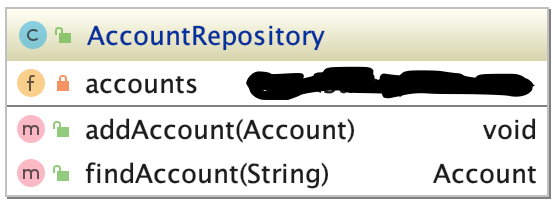
\includegraphics{images/diagrams/accountrepository.png}
  \caption{Klasse AccountRepository}
  \label{fig:content_hierarchy}
\end{figure}


\section{De toepassing uitvoeren}

Alle functionaliteit is nu aanwezig om de toepassing uit te voeren. 
Om de applicatie te starten, run je de main-methode in de klasse \textbf{StreamingServiceAppStarter}.

Eerst zal je een account moeten aanmaken. We gaan ervan uit dat de gebruiker alle informatie netjes invult. Vanaf volgend hoofdstuk gaan we onze toepassing robuuster maken en zorgen dat een foutieve ingave netjes wordt afgehandeld. 

Nadat de account is geregistreerd kan de gebruiker inloggen. Afhankelijk van de geboortdatum die je invult voor het kijkersprofiel (door op de profiel-image te klikken) krijg je aangepaste content te zien.

Als alles correct werkt ben je klaar om te starten met het volgende hoofdstuk!



\end{document}

